\documentclass[a4paper, 14pt]{article}
\usepackage[T2A]{fontenc}
\usepackage[utf8]{inputenc}
\usepackage[english,russian]{babel}
\usepackage[top = 2cm, bottom = 2 cm]{geometry}
\usepackage{cmap}
\usepackage{graphicx}
\usepackage{listings}
\usepackage{color}
\usepackage{amsmath}
\usepackage{pgfplots}
\usepackage{url}
\usepackage{tikz}
\usepackage{float}
\usepackage{multirow}

\usepackage{titlesec}
\titleformat*{\section}{\LARGE\bfseries}
\titleformat*{\subsection}{\Large\bfseries}
\titleformat*{\subsubsection}{\large\bfseries}
\titleformat*{\paragraph}{\large\bfseries}
\titleformat*{\subparagraph}{\large\bfseries}

\begin{document}

	\textbf{Цель работы:} Получение навыков проведения исследований компьютерной математической модели, построенной на квазилинейном уравнении параболического типа. \\
	
	Исследование проводится  с помощью программы, созданной   в лабораторной работе №4. 
	
	
	\subsection*{Исходные данные}
	
\begin{enumerate}
\item Задана математическая модель.\\
Уравнение для функции $T(x)$
$$\frac{d}{dx}(k(x) \frac{dT}{dx}) - \frac{2}{R}\alpha(x)T + \frac{2T_0}{R} \alpha(x) = c(T) \frac{dT}{dt}$$
\item Краевые условия 
$$\begin{cases}
t = 0, T(x,0) = T_0
\\
x = 0,  -k(0)\frac{dT}{dx} = F_0,
\\
x = l,  -k(T(l))\frac{dT}{dx} = \alpha_N(T(l) - T_0)
\end{cases}$$
\item Функции  $k(T), \alpha(x), p(x), f(x)$ заданы своими константами
$$k(T) = a_1(b_1+c_1 \cdot T^{m_1})$$
$$\alpha(x) = \frac{c}{x-d}$$
$$p(x) = \frac{2}{R} \cdot \alpha(x)$$
$$f(x) = \frac{2T_0}{R} \cdot \alpha(x)$$
\item Значения параметров (все размерности согласованы)
$$c(T) = a_2 + b_2T^{m_2} - \frac{c_2}{T^2},$$
$$\alpha_1 = 0.0134, \,\, b_1 = 1,\,\, c_1= 4.35 \cdot 10^{-4},\,\, m_1 = 1$$
$$\alpha_2 = 2.049,\,\, b_2 = 0.563\cdot 10^{-3},\,\, c_2= 0.528 \cdot 10^{5}, \,\,m_2 = 1$$
$$\alpha_0 = 0.05$$
$$\alpha_N = 0.01$$
$$l = 10$$
$$T_0 = 300$$
$$R = 0.5 $$
\item Поток тепла $F(t)$ при $x=0$

$$F(t) = \frac{F_{max}}{t_{max}} t e^{- (t/t_{max} - 1)},$$

где $F_{max}$ -- амплитуда импульса потока, $t_{max}$ -- время достижения амплитуды.
\end{enumerate}


\section*{Результаты работы}

\begin{enumerate}
\item Провести исследование по выбору оптимальных шагов по времени и пространству. Шаги должны быть максимально большими при сохранении устойчивости разностной схемы и заданной точности расчета. \\
Рассмотреть влияние на получаемые результаты амплитуды импульса $F_{max}$ и  времени  $t_{max}$  определяют крутизну фронтов и длительность импульса). \\

Примем $F_{max} = 50$ и  $t_{max} = 10$.\\
Для выбора оптимального шага по времени ($\tau$) будем уменьшать шаги и анализировать сходимость, как это было сделано в лабораторной работе №1.

\begin{figure}[H]
        	\begin{center}
        		\includegraphics[scale=0.5]{tau}
        		\caption{Шаг по времени}
        		\label{tau}
        	\end{center}
\end{figure}

Оптимальный шаг $\tau = 0.01$.

Аналогичным образом найдем оптимальный шаг по пространству ($h$):

\begin{figure}[H]
        	\begin{center}
        		\includegraphics[scale=0.5]{h}
        		\caption{Шаг по пространству}
        		\label{h}
        	\end{center}
\end{figure}

Оптимальный шаг $h = 0.01$.

В дальнейшем в ходе работы будут использованы шаги  $\tau = 0.01$ и $h = 0.01$.

\newpage
Рассмотрим влияние на получаемые результаты амплитуды импульса и времени достижения амплитуды.

На рисунке \ref{F50t1} представлен график при значениях $F_{max} = 50$ и  $t_{max} = 1$

\begin{figure}[H]
        	\begin{center}
        		\includegraphics[scale=0.5]{F50t1}
        		\caption{$F_{max} = 50, t_{max} = 1$}
        		\label{F50t1}
        	\end{center}
\end{figure}

На рисунке \ref{F50t10} представлен график при значениях $F_{max} = 50$ и  $t_{max} = 10$.

При изменении $t_{max}$ меняется время импульса и чем больше $t_{max}$, тем дольше стержень получает тепло и тем сильнее нагревается.

\begin{figure}[H]
        	\begin{center}
        		\includegraphics[scale=0.5]{F50t10}
        		\caption{$F_{max} = 50, t_{max} = 10$}
        		\label{F50t10}
        	\end{center}
\end{figure}

\newpage
На рисунке \ref{F100t1} представлен график при значениях $F_{max} = 100$ и  $t_{max} = 1$.

При увеличении $F_{max}$ увеличивается максимальная температура, на которую может нагреться стержень.

\begin{figure}[H]
        	\begin{center}
        		\includegraphics[scale=0.5]{F100t1}
        		\caption{$F_{max} = 100, t_{max} = 1$}
        		\label{F100t1}
        	\end{center}
\end{figure}

\item График зависимости температуры $T(0,t)$  при 3-4 значениях параметров  $a_2$  и/или  $b_2$  теплоемкости. \\

\textit{Справка.} С ростом теплоемкости темп нарастания температуры снижается (так как стержню необходимо больше тепла, чтобы нагреться до той же температуры, что и при меньшей теплоемкости).\\

На рисунке \ref{ab} представлен график, полученный при значениях $F_{max} = 40$ и  $t_{max} = 1$. 

\begin{figure}[H]
        	\begin{center}
        		\includegraphics[scale=0.5]{ab}
        		\caption{График зависимости $T(0,t)$ при различных значениях $a_2$ и $b_2$}
        		\label{ab}
        	\end{center}
\end{figure}

\newpage
\item График зависимости температуры  T(0, t) (т.е. при x = 0) в частотном режиме теплового нагружения. Импульсы следуют один за другим с заданной частотой $\nu$ (частота определяется количеством импульсов в 1 секунду). \\Показать, что при большом количестве импульсов температурное поле начинает в точности воспроизводиться от импульса к импульсу.  \\Продемонстрировать, как по мере роста частоты импульсов размах колебаний температуры уменьшается (вплоть до нуля), т.е. реализуется квазистационарный режим, при котором в торец поступает постоянный поток $F_c = \nu \int^{t_{u}}_0 F(t)dt$. Здесь $t_u$ -- длительность импульса, определяемая как момент времени, когда $\frac{F(t_u)}{F_{max}} \approx 0.05$. Если взять прямоугольные импульсы длительностью $t_u$, т.е. $F(t)=comst=F_0$, то $F_c = \nu \, F_0 \, t_u$.

\textit{Справка.} Полученное температурное поле должно совпасть с результатом расчета $T(x)$  по программе лаб. работы №3 при $F_0=F_c$, разумеется, при всех одинаковых параметрах модели, в частности, вместо $k(T)$ надо использовать $k(x)$  из лаб. работы №3. \\

Примем $F_{max}=50, t_{max}=1$ и будем постепенно увеличивать частоту $\nu$.

\begin{figure}[H]
        	\begin{center}
        		\includegraphics[scale=0.45]{005}
        		\caption{$\nu=0.05$}
        		\label{a2b2}
        	\end{center}
\end{figure}

\begin{figure}[H]
        	\begin{center}
        		\includegraphics[scale=0.45]{01}
        		\caption{$\nu=0.1$}
        		\label{a2b2}
        	\end{center}
\end{figure}

\begin{figure}[H]
        	\begin{center}
        		\includegraphics[scale=0.5]{02}
        		\caption{$\nu=0.2$}
        		\label{a2b2}
        	\end{center}
\end{figure}

\begin{figure}[H]
        	\begin{center}
        		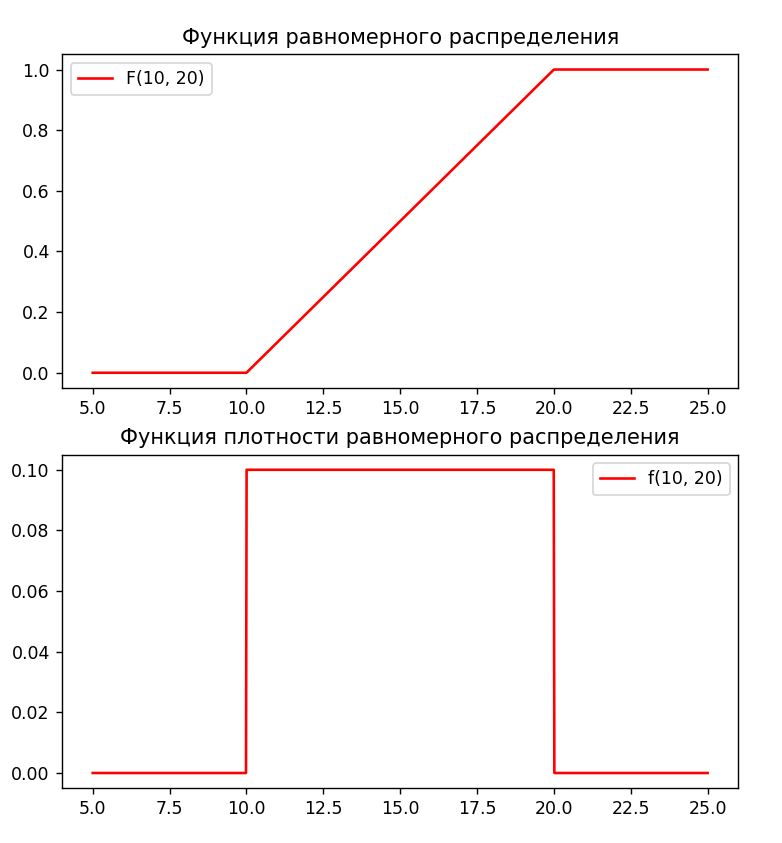
\includegraphics[scale=0.45]{1}
        		\caption{$\nu=1$}
        		\label{a2b2}
        	\end{center}
\end{figure}

\begin{figure}[H]
        	\begin{center}
        		\includegraphics[scale=0.45]{15}
        		\caption{$\nu=50$}
        		\label{a2b2}
        	\end{center}
\end{figure}

На рисунках 7-11 можно наблюдать, что по мере увеличения числа импульсов размах колебаний уменьшается вплоть до нуля.\\

Рассмотрим график, полученный при параметрах модели как в лабораторной работе №3, в частности, при замене $k(T)$ на $k(x)$.

\begin{figure}[H]
        	\begin{center}
        		\includegraphics[scale=0.5]{lab3}
        		\caption{Температурное поле}
        		\label{a2b2}
        	\end{center}
\end{figure}

Полученное температурное поле совпадает с результатом расчетов в лабораторной работе №3.

\end{enumerate}

\section*{Вывод}

В ходе лабораторной работы были получены навыки проведения исследований компьютерной математической модели, построенной на  квазилинейном уравнении параболического типа.

\end{document}